\documentclass[12pt,oneside]{book}
\newcommand{\TITLE}{ CPP}
\usepackage[utf8]{inputenc}
\usepackage[margin=0.5in]{geometry}
\usepackage[usestackEOL]{stackengine}
\usepackage{amsmath , esint,braket,lmodern,mhchem,bohr,lewis,chemfig,draftwatermark,xcolor,graphicx , amssymb ,ragged2e , listings , siunitx , float , eqparbox, centernot , esvect , bm , fancyhdr , fourier-orns}
\usepackage[ddmmyyyy]{datetime}
\usepackage{fourier-orns}
\usepackage{changepage}
\usepackage{bbm}\usepackage{chngcntr}
\usepackage{hyperref}
\usepackage{ifthen}
\usepackage[many]{tcolorbox}
\DeclareMathOperator{\sech}{sech}
\DeclareMathOperator{\csch}{csch}
\DeclareMathOperator{\arcsec}{arcsec}
\DeclareMathOperator{\arccot}{arcCot}
\DeclareMathOperator{\arccsc}{arcCsc}
\DeclareMathOperator{\arccosh}{arcCosh}
\DeclareMathOperator{\arcsinh}{arcsinh}
\DeclareMathOperator{\arctanh}{arctanh}
\DeclareMathOperator{\arcsech}{arcsech}
\DeclareMathOperator{\arccsch}{arcCsch}
\DeclareMathOperator{\arccoth}{arcCoth} 
\DeclareMathOperator{\grad}{\vv{\text{grad}}} 
\DeclareMathOperator{\conj}{^*} 
\DeclareMathOperator{\vect}{vv} 
\DeclareMathOperator{\Vect}{\text{Vect}} 
\DeclareMathOperator{\degree}{c^\circ} 
\DeclareMathOperator{\degre}{^\circ} 
\DeclareMathOperator{\transpose}{^\dagger} 
\DeclareMathOperator{\adjoint}{^\dagger} 

\newcommand{\moyenne}[1]{\langle #1 \rangle} 
\newcommand{\lagrange}{\mathcal{L}}
\newcommand{\fourier}{\mathcal{F}}
\newcommand{\hilbert}{\mathcal{H}}
\newcommand{\p}{\mathcal{P}}
\newcommand{\x}{\chi}
\newcommand{\ve}[1]{\vv{#1}}
\newcommand{\push}[1]{\begin{adjustwidth}{5mm}{}#1\end{adjustwidth}}
\newcommand{\operator}[1]{\widehat{#1}}
\newcommand{\HRule}{\rule{\linewidth}{0.5mm}} % Defines a new command for the horizontal lines, change thickness here
\renewcommand{\chaptermark}[1]{\markboth{\MakeUppercase{#1}}{}}
\renewcommand{\headrule}{%
\vspace{-8pt}\hrulefill
\raisebox{-2.1pt}{\quad\decofourleft\decotwo\decofourright\quad}\hrulefill}
\definecolor{myred}{RGB}{255, 14, 0}
\everymath{\displaystyle}

\def\changemargin#1{\list{}{\leftmargin#1}\item[]}
\let\endchangemargin=\endlist 

\makeatletter
\newcommand*{\rom}[1]{\expandafter\@slowromancap\romannumeral #1@}%roman numbers
\makeatother

%hyperlink shit

\hypersetup{
    colorlinks,
    citecolor=black,
    filecolor=black,
    linkcolor=black,
    urlcolor=black
}
% Table specail cell , it's for making line break in table cell
\newcommand{\specialcell}[2][c]{%
  \begin{tabular}[#1]{@{}c@{}}#2\end{tabular}}

  \definecolor{main}{HTML}{5989cf}    % setting main color to be used
\definecolor{sub}{HTML}{cde4ff}     % setting sub color to be used

\tcbset{
    sharp corners,
    colback = white,
    before skip = 0.2cm,    % add extra space before the box
    after skip = 0.5cm      % add extra space after the box
}   
\newtcolorbox{boxH}{
    colback = sub, 
    colframe = main, 
    boxrule = 0pt, 
    leftrule = 6pt % left rule weight
}
\newtcolorbox{gpt}{
    sharpish corners, % better drop shadow
    boxrule = 0pt,
    toprule = 4.5pt, % top rule weight
    enhanced,
    fuzzy shadow = {0pt}{-2pt}{-0.5pt}{0.5pt}{black!35} % {xshift}{yshift}{offset}{step}{options} 
}
\definecolor{codegreen}{rgb}{0,0.6,0}
\definecolor{codegray}{rgb}{0.5,0.5,0.5}
\definecolor{codepurple}{rgb}{0.58,0,0.82}
\definecolor{backcolour}{rgb}{0.95,0.95,0.92}

\lstdefinestyle{mystyle}{
    backgroundcolor=\color{backcolour},   
    commentstyle=\color{codegreen},
    keywordstyle=\color{magenta},
    numberstyle=\tiny\color{codegray},
    stringstyle=\color{codepurple},
    basicstyle=\ttfamily\footnotesize,
    breakatwhitespace=false,         
    breaklines=true,                 
    captionpos=b,                    
    keepspaces=true,                 
    numbers=left,                    
    numbersep=5pt,                  
    showspaces=false,                
    showstringspaces=false,
    showtabs=false,                  
    tabsize=2,
    basicstyle = \small
}

\lstset{style=mystyle}
\SetWatermarkAngle{45} 
\SetWatermarkLightness{.99} 
\SetWatermarkFontSize{0.1cm} 
\SetWatermarkScale{0} 
\SetWatermarkText{supahaka}


\begin{document}
\renewcommand {\NOTICEE}{ Based on the tutorial at cplusplus.com -2023}
\pagestyle{fancy}
\fancyhf{}
\fancyfoot[R]{Tenji$_\text{org}$}
\fancyfoot[C]{\thepage}
\fancyfoot[L]{\tiny www.tenji.org}
\fancyhead[RO]{\nouppercase{\leftmark\hfill\TITLE}}


\DraftwatermarkOptions{stamp=false}
    \begin{titlepage}
        \begin{center}
            \vspace*{5cm}
            \Huge
            \HRule \\[0.4cm]
            \textbf{Project Tenji: \\ \TITLE}\\
            \Large 
            \HRule \\[1.5cm]
            \vspace{2cm}
            \vfill
        \end{center}
        \vfill
        { \scriptsize Project Tenji \copyright 2024 by Khalil Salahat and Mohamad El Moussawi  \\}
        { \scriptsize Hosted at tenji.org , contact : contact@tenji.org \\}
        { \scriptsize \NOTICEE  \\}
    \end{titlepage} 
    \tableofcontents
\DraftwatermarkOptions{stamp=true}
\chapter{Basics}
\section{Fundamental data types}
\begin{tabular}{|l|l|l|l|}
	\hline
	Name        & Description                                  & \specialcell{Size                                                                               \\ in bytes} & Range                                                                       \\ \hline
	char        & Charcter or small integer                    & 1                 & \specialcell{ signed: -128 to 127                                           \\unsigned: 0 to 255}\\ \hline
	short int   & Short Integer.                               & 2                 & \specialcell{ signed: -32768 to 32767                                       \\unsigned: 0 to 65535}\\ \hline
	int         & Integer.                                     & 4                 & \specialcell{ signed: -2147483648 to 2147483647                             \\unsigned: 0 to 4294967295 }\\ \hline
	long int    & Long integer.                                & 4                 & \specialcell{ signed: -2147483648 to 2147483647                             \\unsigned: 0 to 4294967295 }\\ \hline
	bool        & Boolean value.                               & 1                 & \specialcell{ true or false                                               } \\ \hline
	float       & Floating point number.                       & 4                 & \specialcell{ +/- 3.4e +/- 38 (~7 digits)                                 } \\ \hline
	double      & Double precision floating point number.      & 8                 & \specialcell{ +/- 1.7e +/- 308 (~15 digits)                               } \\ \hline
	long double & Long double precision floating point number. & 8                 & \specialcell{ +/- 1.7e +/- 308 (~15 digits)                               } \\ \hline
	wchar\_t    & Wide character.                              & 2 or 4            & \specialcell{ 1 wide character                                            } \\ \hline
\end{tabular}
Wide characters are used mainly to represent non-English or exotic character sets.
\section{Declaration and initialization of variables}
 \begin{lstlisting}[language=C++]
int a ;
float mynumber;
int a, b, c; // to declare more than one variable of the same type
unsigned short int Number; // to declare variable with type   

int a=5; // initial value = 5
int b(2); // initial value = 2
\end{lstlisting}
\pagebreak
\section{Scope of variables}

\begin{minipage}{0.6\linewidth}
    A variable can be either of global or local scope. A global variable is a variable declared in the main body of the source code, outside all functions, while a local variable is one declared within the body of a function or a block.
\end{minipage}
\begin{minipage}{0.4\linewidth}
    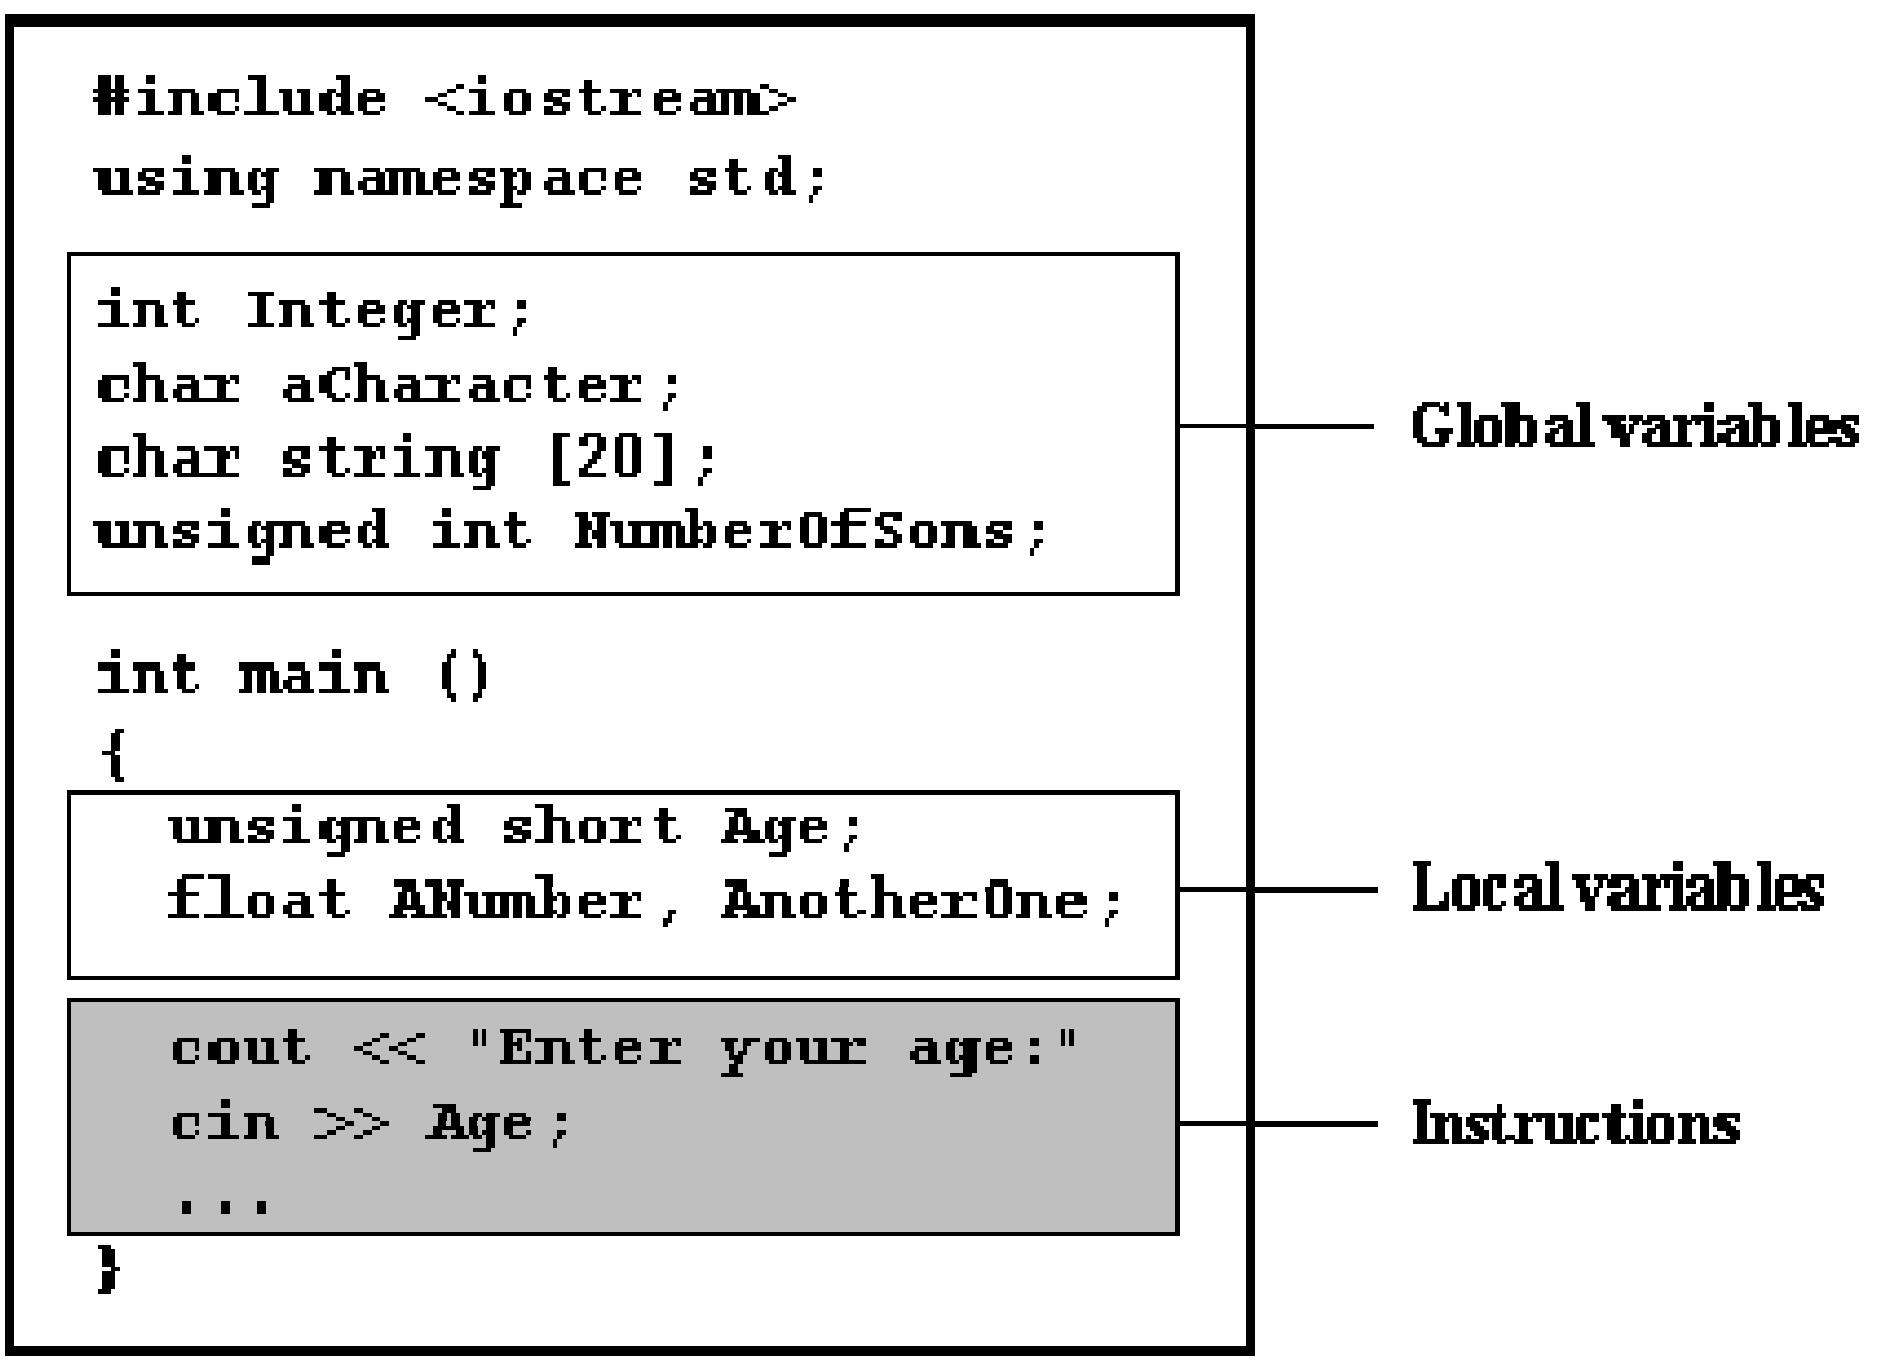
\includegraphics[width=\linewidth]{../pic/3316/22.png}
\end{minipage}

\section{Intro to strings}
We need to include an additional header file in our source code: $<$string$>$ and have access to the std namespace .\\
Declaration and initialization :
\begin{lstlisting}[language=C++]
string mystring = "This is a string";
string mystring ("This is a string");
\end{lstlisting}
\section{Constants}
Constants are expressions with a fixed value.
\subsection{Literals}
Literals are used to express particular values within the source code of a program.
\subsubsection{Integer Numerals}
They are numerical constants that identify integer decimal values.\\
In addition to decimal numbers (base 10) C++ allows the use as literal constants of octal numbers (base 8) and hexadecimal numbers (base 16).
	\begin{lstlisting}[language=C++]
75 // decimal
0113 // octal start with 0
0x4b // hexadecimal start with 0x
\end{lstlisting}
Literal constants, like variables, are considered to have a specific data type.
	\begin{lstlisting}[language=C++]
75 // int
75u // unsigned int
75l // long
75ul // unsigned long
\end{lstlisting}
\subsubsection{Floating Point Numbers}
They express numbers with decimals and/or exponents.
	\begin{lstlisting}[language=C++]
3.14159 // 3.14159
6.02e23 // 6.02 x 10^23
1.6e-19 // 1.6 x 10^-19
3.0 // 3.0

3.14159L // long double
6.02e23f // float
\end{lstlisting}
\subsubsection{Character and string literals}
There also exist non-numerical constants, like:
\begin{lstlisting}[language=C++]
'z'
'p'
"Hello world"
"How do you do?"
\end{lstlisting}
Character and string literals have certain peculiarities, like the escape codes.\\ These are special characters that are difficult or impossible to express otherwise in the source code of a program:
\begin{center}
	\begin{tabular}{|l|l|}
		\hline
		$\backslash$n          & newline                 \\ \hline
		$\backslash$r          & carriage return         \\ \hline
		$\backslash$t          & tab                     \\ \hline
		$\backslash$v          & vertical tab            \\ \hline
		$\backslash$b          & backspace               \\ \hline
		$\backslash$f          & form feed (page feed)   \\ \hline
		$\backslash$a          & alert (beep)            \\ \hline
		$\backslash$'          & single quote(')         \\ \hline
		$\backslash$"          & double quote(")         \\ \hline
		$\backslash$?          & question mark (?)       \\ \hline
		$\backslash\backslash$ & backslash($\backslash$) \\ \hline
	\end{tabular}
\end{center}
\begin{itemize}
	\item String literals can extend to more than a single line of code by putting a backslash sign ($\backslash$) at the end of each unfinished line.
		      \begin{lstlisting}[language=C++]
        "string expressed in \
    two lines" 
    \end{lstlisting}
	\item You can also concatenate several string constants separating them by one or several blank spaces, tabulators, newline or any other valid blank character:
	      \begin{lstlisting}[language=C++]
            "this forms" "a single"     " string "
            "of characters"
    \end{lstlisting}
	\item Finally, if we want the string literal to be explicitly made of wide characters (wchar\_t), instead of narrow characters
	      (char), we can precede the constant with the L prefix:
	      \begin{lstlisting}[language=C++]
        L"This is a wide character string"
    \end{lstlisting}
\end{itemize}
\subsubsection{Boolean literals}
There are only two valid Boolean values: true and false. These can be expressed in C++ as values of type bool by
using the Boolean literals true and false.
\subsection{Defined constants}
ou can define your own names for constants that you use very often without having to resort to memory-consuming variables, simply by using the \#define preprocessor directive. Its format is:
\begin{lstlisting}[language=C++]
#define PI 3.14159
#define NEWLINE '\n'
\end{lstlisting}
\subsection{Declared constants}
With the const prefix you can declare constants with a specific type in the same way as you would do with a variable:
\begin{lstlisting}[language=C++]
    const int pathwidth = 100; 
    const char tabulator = '\t';
\end{lstlisting}
\section{Operators}
\subsection{Assignment (=)}
The assignment operator assigns a value to a variable.\\
The assignment operation always takes place from right to left, and never the other way.
	\begin{lstlisting}[language=C++]
        a=5;
        a=b;
    \end{lstlisting}
the assignment operation can be used as the value (or part of an value) for another assignment operation.
	\begin{lstlisting}[language=C++]
        a = 2+(b=5);
    \end{lstlisting}
is equivalent to :
\begin{lstlisting}[language=C++]
        b =5 ;
        a = 2 + b;
    \end{lstlisting}
you cans assign a value to multiple variables :
\begin{lstlisting}[language=C++]
        a = b = c = 5;
    \end{lstlisting}
\subsection{Arithmetic operators ( +,-,*,/,\%)}
\begin{tabular}{|l|l|}
	\hline
	+  & addition       \\ \hline
	-  & subtraction   \\ \hline
	*  & multiplication \\ \hline
	/  & division       \\ \hline
	\% & modulo         \\ \hline
\end{tabular}
Modulo is the operation that gives the remainder of a division of two values.
\subsection{Increase an decrease (++,--)}
The increase operator (++) and the decrease operator (--) increase or reduce by one the value stored in a variable.Thus:
\begin{lstlisting}[language=C++]
    c++;
    c+=1;
    c=c+1;
\end{lstlisting}
are all equivalent.\\
A characteristic of this operator is that it can be used both as a prefix (++a) and as a suffix(a++).Notice the difference :
\begin{lstlisting}[language=C++]
    // Case 1
    b =3 ;
    a = ++b;// a contains 4, b contains 4
    // Case 2
    b =3 ;
    a = b ++;// acontains 3, b contais 4
\end{lstlisting}
\subsection{Relational and equality operators ( ==, !=,$ >, <, >=, <=$ )}
In order to evaluate a comparison between two expressions we can use the relational and equality operators.
\begin{center}
	\begin{tabular}{|l|l|l|l|l|}
		\hline
		==   & Equal to              \\ \hline
		!=   & Note equal to         \\ \hline
		$>$  & Greater than          \\ \hline
		$<$  & Less than or equal to \\ \hline
		$<=$ & Less than or equal to \\ \hline
	\end{tabular}
\end{center}
\subsection{Logical operators (!,\&\&,$||$)}
\subsubsection{! operator}
The Operator ! is the C++ operator to perform the Boolean operation NOT.
	\begin{lstlisting}[language=C++]
    !true // evaluates to false
    !false // evaluates to true. 
\end{lstlisting}
\subsubsection{\&\& operator}
\begin{center}
	\begin{tabular}{|l|l|l|}
		\hline
		a     & b     & a\&\&b \\ \hline
		true  & true  & true   \\ \hline
		true  & false & false  \\ \hline
		false & true  & false  \\ \hline
		false & false & false  \\ \hline
	\end{tabular}
\end{center}
\subsubsection{$||$ operator}
\begin{center}
	\begin{tabular}{|l|l|l|}
		\hline
		a     & b     & a$||$b \\ \hline
		true  & true  & true   \\ \hline
		true  & false & true   \\ \hline
		false & true  & true   \\ \hline
		false & false & false  \\ \hline
	\end{tabular}
\end{center}
\subsubsection{Conditional operator (?)}
The conditional operator evaluates an expression returning a value if that expression is true and a different one if the expression is evaluated as false. Its format is:
\begin{lstlisting}[language=C++]
    condition ? result1 : result2
\end{lstlisting}
If condition is true the expression will return result1, if it is not it will return result2.
\subsection{Comma operator ( , )}
The comma operator (,) is used to separate two or more expressions that are included where only one expression is expected.
	\begin{lstlisting}[language=C++]
    a = (b=3, b+2);
\end{lstlisting}
Would first assign the value 3 to b, and then assign b+2 to variable a. So, at the end, variable a would contain the value 5 while variable b would contain value 3.
\subsection{Bitwise operators}
\begin{tabular}{|l|l|l|}
	\hline
	\&       & AND & Bitwise AND                      \\ \hline
	|        & OR  & Bitwise Inclusive OR             \\ \hline
	$\hat{}$ & XOR & Bitwise Exclusive OR             \\ \hline
	$\sim$   & NOT & Unary complement (bit inversion) \\ \hline
	$<<$     & SHL & Shift Left                       \\ \hline
	$>>$     & SHR & Shift Right                      \\ \hline
\end{tabular}
\subsection{Explicit type casting oerator}
Type casting operators allow you to convert a datum of a given type to another.
	\begin{lstlisting}[language=C++]
int i; 
float f = 3.14;
i = (int) f; 
// OR
i = int ( f );
\end{lstlisting}
\subsection{sizeof()}
This operator accepts one parameter, which can be either a type or a variable itself and returns the size in bytes of that type or object:
\begin{lstlisting}[language=C++]
a = sizeof (char);
\end{lstlisting}
\subsection{Precedence of operators }
\begin{tabular}{|l|l|l|l|}
	\hline
	\specialcell{Level} & \specialcell{Operator}                                    & \specialcell{Description}       & \specialcell{Grouping}      \\ \hline
	\specialcell{1}     & \specialcell{::}                                          & \specialcell{scope}             & \specialcell{Left-to-right} \\ \hline
	\specialcell{2}     & \specialcell{() [] . $->$ ++ --}                          & \specialcell{postfix}           & \specialcell{Left-to-right} \\ \hline
	\specialcell{3}     & \specialcell{++ -- $\sim$ sizeof new delete                                                                               \\ * \& \\ +-}  &\specialcell{ unary (prefix)\\indirection and reference (pointers)\\unary sign operator}  &\specialcell{Right-to-left}   \\ \hline
	\specialcell{4}     & \specialcell{(type)}                                      & \specialcell{type casting}      & \specialcell{Right-to-left} \\ \hline
	\specialcell{5}     & \specialcell{.* $->$*}                                    & \specialcell{pointer-to-member} & \specialcell{Left-to-right} \\ \hline
	\specialcell{6}     & \specialcell{* / \%}                                      & \specialcell{multiplicative}    & \specialcell{Left-to-right} \\ \hline
	\specialcell{7}     & \specialcell{+ -}                                         & \specialcell{additive}          & \specialcell{Left-to-right} \\ \hline
	\specialcell{8}     & \specialcell{$<< >>$}                                     & \specialcell{shift}             & \specialcell{Left-to-right} \\ \hline
	\specialcell{9}     & \specialcell{$< > <= >=$}                                 & \specialcell{relational}        & \specialcell{Left-to-right} \\ \hline
	\specialcell{10}    & \specialcell{$== !=$}                                     & \specialcell{equality}          & \specialcell{Left-to-right} \\ \hline
	\specialcell{11}    & \specialcell{\&}                                          & \specialcell{bitwise AND}       & \specialcell{Left-to-right} \\ \hline
	\specialcell{12}    & \specialcell{$\hat{}$}                                    & \specialcell{bitwise XOR}       & \specialcell{Left-to-right} \\ \hline
	\specialcell{13}    & \specialcell{$|$}                                         & \specialcell{bitwise OR}        & \specialcell{Left-to-right} \\ \hline
	\specialcell{14}    & \specialcell{\&\&}                                        & \specialcell{logical AND}       & \specialcell{Left-to-right} \\ \hline
	\specialcell{15}    & \specialcell{$||$}                                        & \specialcell{logical OR}        & \specialcell{Left-to-right} \\ \hline
	\specialcell{16}    & \specialcell{?:}                                          & \specialcell{conditional}       & \specialcell{Right-to-left} \\ \hline
	\specialcell{17}    & \specialcell{= *= /= \%= += -= $>>= << = \&= \hat{}= |=$} & \specialcell{assignemnt}        & \specialcell{Right-to-left} \\ \hline
	\specialcell{18}    & \specialcell{,}                                           & \specialcell{comma}             & \specialcell{Left-to-right} \\ \hline
\end{tabular}\\
All these precedence levels for operators can be manipulated or become more legible by removing possible ambiguities using parentheses ()
\section{Basic Input/Output}
\subsection{Standard Output (cout)}
By default, the standard output of a program is the screen, and the C++ stream object defined to access it is cout.
cout is used in conjunction with the insertion operator $<<$
\begin{lstlisting}[language=C++]
cout << "Output sentence"; // prints Output sentence on screen
cout << 120; // prints number 120 on screen
cout << x; // prints the content of x on screen
\end{lstlisting}
The $<<$ operator inserts the data that follows it into the stream preceding it.\\
The insertion operator ($<<$) may be used more than once in a single statement:
\begin{lstlisting}[language=C++]
    cout << "Hello, I am " << age << " years old and my zipcode is " << zipcode;
\end{lstlisting}
In C++ a new-line character can be specified as $\backslash$n\\
Additionally, to add a new-line, you may also use the endl manipulator.
	\begin{lstlisting}[language=C++]
    cout << "First sentence." << endl; 
\end{lstlisting}
\subsection{Standard Input (cin)}
The standard input device is usually the keyboard.. Handling the standard input in C++ is done by applying the
overloaded operator of extraction (>>) on the cin stream. The operator must be followed by the variable that will
store the data that is going to be extracted from the stream.
	\begin{lstlisting}[language=C++]
int age;
cin >> age;
\end{lstlisting}
You can also use cin to request more than one datum input from the user:
\begin{lstlisting}[language=C++]
cin >> a >> b;
// same as
cin >> a;
cin >> b;
\end{lstlisting}
\subsubsection{cin and strings}
We can use cin to get strings.However,cin extraction stops reading as soon as if finds any blank space character.\\
In order to get entire lines, we can use the function getline, which is the more recommendable way to get user
input with cin:
\begin{lstlisting}[language=C++]
getline (cin, mystr)
\end{lstlisting}
The standard header file $<$sstream$>$ defines a class called stringstream that allows a string-based object to be treated as a stream.This way we can perform extraction or insertion operations from/to strings,For example, if we want to extract an integer from a
string we can write:
\begin{lstlisting}[language=C++]
    string mystr ("1204"); 
    int myint; 
    stringstream(mystr) >> myint;
\end{lstlisting}
\chapter{Control Structures}
\section{Control Structures}
A program is usually not limited to a linear sequence of instructions. During its process it may bifurcate, repeat code or take decisions.
\subsection{block \{\}}
A block is a group of statements which are separated by semicolons (;) like all C++ statements, but grouped together in a block enclosed in braces: { }:
\begin{lstlisting}[language=C++]
{statement1;statement2; statement3;}
\end{lstlisting}
\subsection{Conditional structure:if and else}
The if keyword is used to execute a statement or block only if a condition is fulfilled.
	\begin{lstlisting}[language=C++]
    if(condition) statement
\end{lstlisting}
Where condition is the expression that is being evaluated. If this condition is true, statement is executed. If it is false, statement is ignored.\\
We can additionally specify what we want to happen if the condition is not fulfilled by using the keyword else.
	\begin{lstlisting}[language=C++]
    if (condition) statement1 else statement2
\end{lstlisting}
The if + else structures can be concatenated with the intention of verifying a range of values.
	\begin{lstlisting}[language=C++]
if (x > 0) 
 cout << "x is positive";
else if (x < 0) 
 cout << "x is negative";
else
 cout << "x is 0"; 
\end{lstlisting}
\subsection{Iteration structures (loops)}
Loops have as purpose to repeat a statement a certain number of times or while a condition is fulfilled.
\subsubsection{The while loop}
format :
\begin{lstlisting}[language=C++]
    while (expression) statement
\end{lstlisting}
And its functionality is simply to repeat statement while the condition set in expression is true.
\subsubsection{The do-while loop}
format :
\begin{lstlisting}[language=C++]
    do statement while (condition);
\end{lstlisting}
Its functionality is exactly the same as the while loop, except that condition in the do-while loop is evaluated after the execution of statement instead of before.
\subsubsection{The for loop}
format :
\begin{lstlisting}[language=C++]
    for (initialization; condition; increase) statement;
\end{lstlisting}
And its main function is to repeat statement while condition remains true, like the while loop. But in addition, the for loop provides specific locations to contain an initialization statement and an increase statement.\\
Note that
\begin{itemize}
	\item The initialization and increase fields are optional.
	\item Optionally, using the comma operator (,) we can specify more than one expression in any of the fields included in a for loop
\end{itemize}
\subsection{Jump statements}
\subsubsection{The break statement}
Using break we can leave a loop even if the condition for its end is not fulfilled. It can be used to end an infinite loop, or to force it to end before its natural end.
	\begin{lstlisting}[language=C++]
    break;
\end{lstlisting}
\subsubsection{The continue statement}
The continue statement causes the program to skip the rest of the loop in the current iteration as if the end of the statement block had been reached, causing it to jump to the start of the following iteration.
	\begin{lstlisting}[language=C++]
    continue;
\end{lstlisting}
\subsubsection{The goto statement}
goto allows to make an absolute jump to another point in the program.The destination point is identified by a label, which is then used as an argument for the goto statement. A label is
made of a valid identifier followed by a colon (:).\\
example :
\begin{lstlisting}[language=C++]
include <iostream>
using namespace std; 
int main () 
{ 
 int n=10; 
 loop: 
 cout << n << ", "; 
 n--; 
 if (n>0) goto loop; 
 cout << "FIRE!\n"; 
 return 0; 
} 
\end{lstlisting}
\subsubsection{The exit function}
The purpose of exit is to terminate the current program with a specific exit code.
	\begin{lstlisting}[language=C++]
    void exit (int exitcode);
\end{lstlisting}
\subsection{The selective structure: switch}
Its objective is to check several possible constant values for an expression.
	\begin{lstlisting}[language=C++]
switch (expression) 
{ 
 case constant1: 
 group of statements 1; 
 break; 
 case constant2: 
 group of statements 2; 
 break; 
 . 
 . 
 . 
 default: 
 default group of statements 
} 
\end{lstlisting}
\begin{itemize}
	\item switch evaluates expression and checks if it is equivalent to constant1, if it is, it
	      executes group of statements 1 until it finds the break statement. When it finds this break statement the
	      program jumps to the end of the switch selective structure.
	\item If expression was not equal to constant1 it will be checked against constant2. If it is equal to this, it will execute
	      group of statements 2 until a break keyword is found, and then will jump to the end of the switch selective
	      structure.
	\item Finally, if the value of expression did not match any of the previously specified constants the program will execute the statements included after the default: label, if it exists
\end{itemize}
\section{Function}
Using functions we can structure our programs in a more modular way.\\
A function is a group of statements that is executed when it is called from some point of the program.
	\begin{lstlisting}[language=C++]
    type name ( parameter1, parameter2, ...) { statements }
\end{lstlisting}
\begin{itemize}
	\item type is the data type specifier of the data returned by the function, if we want to return no value we use the void type specifier.
	\item name is the identifier by which it will be possible to call the function.
	\item parameters :Each parameter consists of a data type specifier followed by an identifier, like any regular variable declaration (for example: int x) and which acts within the function as a regular local variable. They allow to pass arguments to the function when it is called. The different parameters are separated by commas.
	\item statements is the function's body. It is a block of statements surrounded by braces \{ \}.
\end{itemize}
the format for calling a function includes specifying its name and enclosing its parameters between parentheses.
	\begin{lstlisting}[language=C++]
    printmessage();
\end{lstlisting}
\subsection{Arguments passed by value and by reference}
\begin{itemize}
	\item Passing by value :\\
	      This means that when calling a function with parameters, what we have passed to the function were copies of their values but never the variables themselves.
	      \begin{center}
		      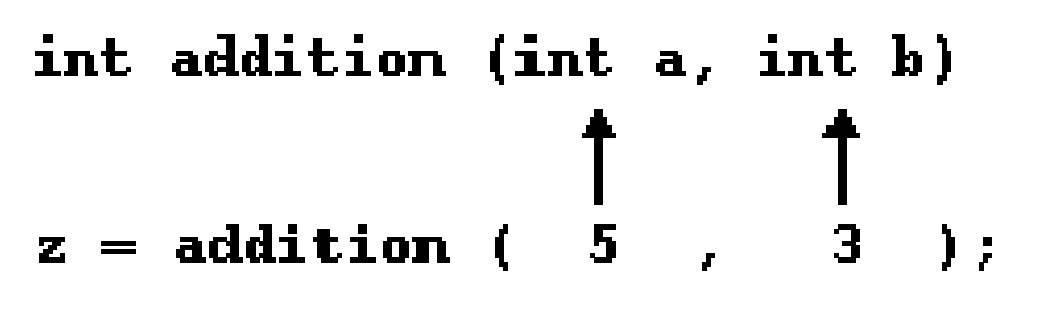
\includegraphics[width=0.3\linewidth]{../pic/3316/24.png}
	      \end{center}
	\item Passing by reference:\\
	      When a variable is passed by reference we are not passing a copy of its value, but we are somehow passing the
	      variable itself to the function and any modification that we do to the local variables will have an effect in their
	      counterpart variables passed as arguments in the call to the function. \\
	      to pass by reference the type of each parameter was followed by an ampersand sign ($\&$)
	      \begin{center}
		      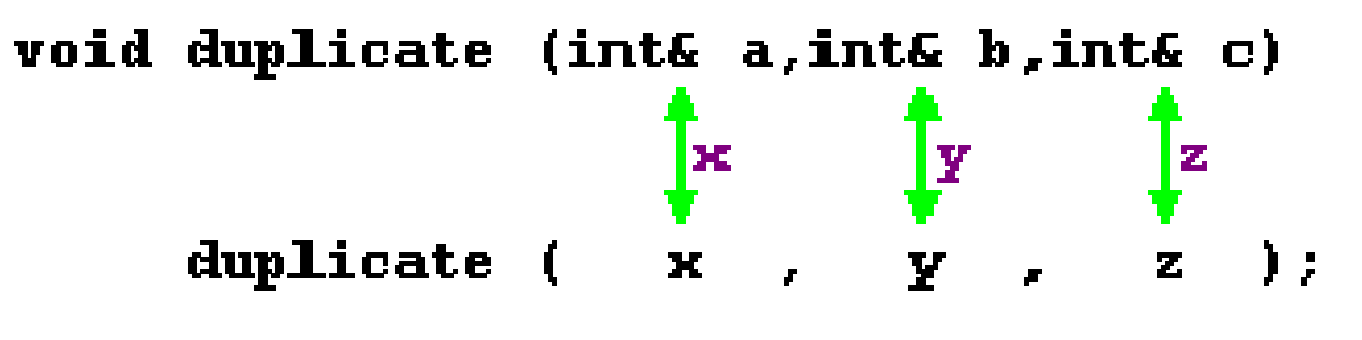
\includegraphics[width=0.3\linewidth]{../pic/3316/23.png}
	      \end{center}
\end{itemize}
\subsection{Default values in parameters}
When declaring a function we can specify a default value for each of the last parameters. This value will be used if the corresponding argument is left blank when calling to the function.
	\begin{lstlisting}[language=C++]
    int divide (int a, int b=2){
        ...
    }
\end{lstlisting}
\subsection{Overloaded functions}
In C++ two different functions can have the same name if their parameter types or number are different.
	\begin{lstlisting}[language=C++]
#include <iostream>
using namespace std; 
int operate (int a, int b) 
{ 
 return (a*b); 
} 
float operate (float a, float b) 
{ 
 return (a/b); 
} 
int main () 
{ 
 int x=5,y=2; 
 float n=5.0,m=2.0; 
 cout << operate (x,y); 
 cout << "\n"; 
 cout << operate (n,m); 
 cout << "\n"; 
 return 0; 
} 
\end{lstlisting}
\subsection{Recursivity}
Recursivity is the property that functions have to be called by themselves.
	\begin{lstlisting}[language=C++]
long factorial (long a) 
{ 
 if (a > 1) 
 return (a * factorial (a-1)); 
 else
 return (1); 
} 
    \end{lstlisting}
\subsection{Declaring functions}
To be able to call a function it must have been declared in some earlier point of the code.\\
There is an alternative way to avoid writing the whole code of a function before it can be used.\\
This can be achieved by declaring just a prototype of the function before it is used, instead of the entire definition.
	\begin{lstlisting}[language=C++]
    type name ( argument_type1, argument_type2, ...);
\end{lstlisting}
Having the prototype of all functions together in the same place within the source code is found practical by some
programmers, and this can be easily achieved by declaring all functions prototypes at the beginning of a program.
\chapter{Compound data types }
\section{Arrays}
An array is a series of elements of the same type placed in contiguous memory locations that can be individually referenced by adding an index to a unique identifier.
	\begin{lstlisting}[language=C++]
    type name [elements];
\end{lstlisting}
where  elements field specifies how many of these elements the array has to contain.
\subsection{Initializing arrays}
we have the possibility to assign initial values to each one of its elements by enclosing the values in braces \{ \}
\begin{lstlisting}[language=C++]
    int billy [5] = { 16, 2, 77, 40, 12071 };
    // OR
    int billy [] = { 16, 2, 77, 40, 12071 };
\end{lstlisting}
\begin{center}
	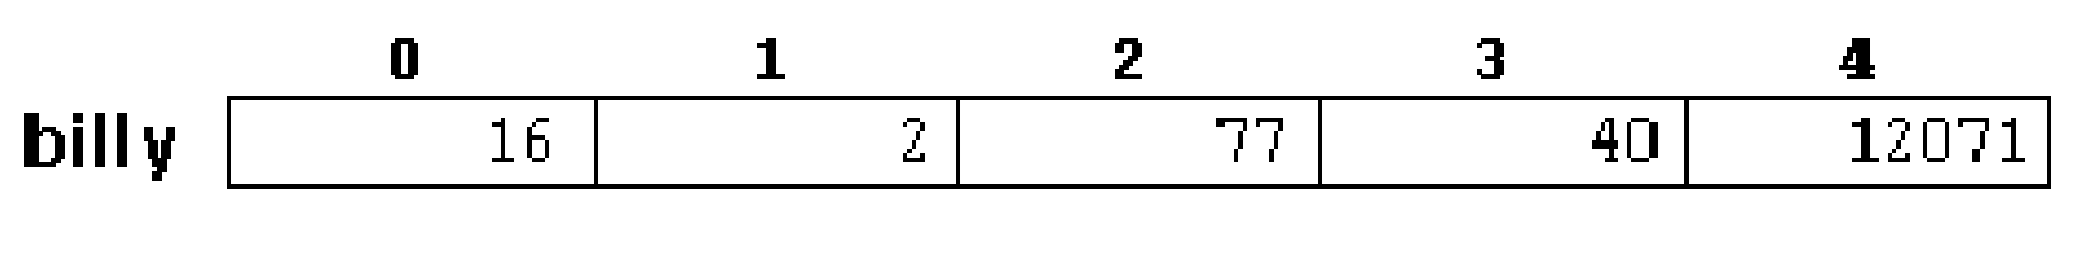
\includegraphics[width=0.5\linewidth]{../pic/3316/25.png}
\end{center}
\subsection{Accessing the values of an array}
In any point of a program in which an array is visible, we can access the value of any of its elements individually as if it was a normal variable, thus being able to both read and modify its value.
	\begin{lstlisting}[language=C++]
    name [index]
\end{lstlisting}
\begin{center}
	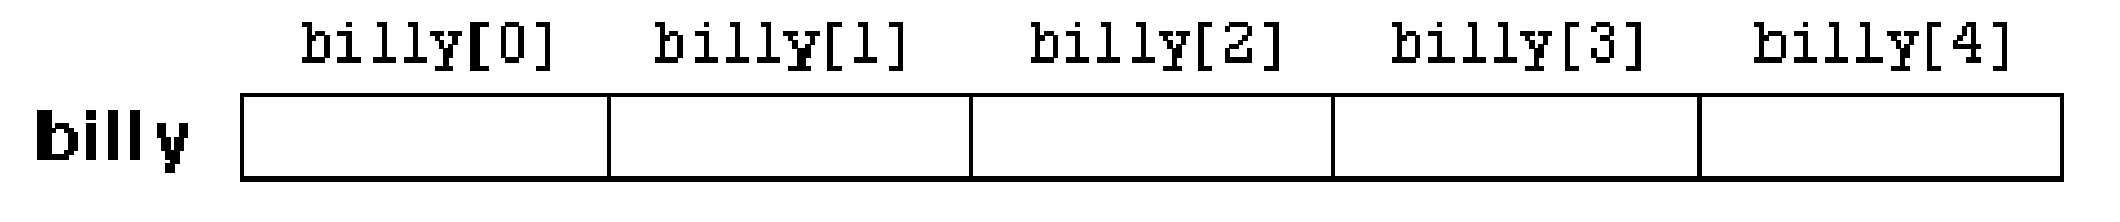
\includegraphics[width=0.5\linewidth]{../pic/3316/26.png}
\end{center}
\begin{lstlisting}[language=C++]
    billy[2] = 75;// To store a value 
    a = billy[2]; // to pass the value to a variable
\end{lstlisting}
\subsection{Multidimensional arrays}
Multidimensional arrays can be described as "arrays of arrays".
\begin{center}
	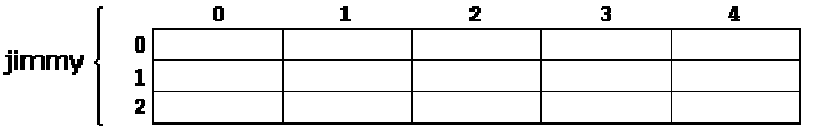
\includegraphics[width=0.5\linewidth]{../pic/3316/27.png}\\
	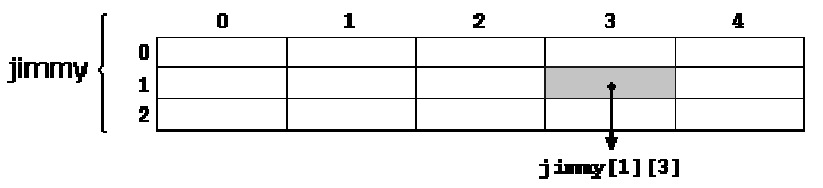
\includegraphics[width=0.5\linewidth]{../pic/3316/28.png}
\end{center}
declaration:
\begin{lstlisting}[language=C++]
    int jimmy [3][5];// declaration 
    jimmy[1][2];// accessing 
\end{lstlisting}
\subsection{Arrays as parameters}
In C++ it is not possible to pass a complete block of memory by value as a parameter to a function, but we are allowed to pass its address.
declaration :
\begin{lstlisting}[language=C++]
    void procedure (int arg[])
\end{lstlisting}
In a function declaration it is also possible to include multidimensional arrays.
	\begin{lstlisting}[language=C++]
    base_type[][depth][depth]
\end{lstlisting}
Notice that the first brackets [] are left blank while the following ones are not. This is so because the compiler must be able to determine within the function which is the depth of each additional dimension.
\section{Character Sequences}
because strings are in fact sequences of characters, we can represent them also as plain arrays of char elements.\\
since the array of characters can store shorter sequences than its total length, a special character is used to signal the end of the valid sequence: the null character, whose literal constant can be written as '$\backslash$0'\\
\begin{lstlisting}[language=C++]
    char jenny [20];
\end{lstlisting}
\begin{center}
	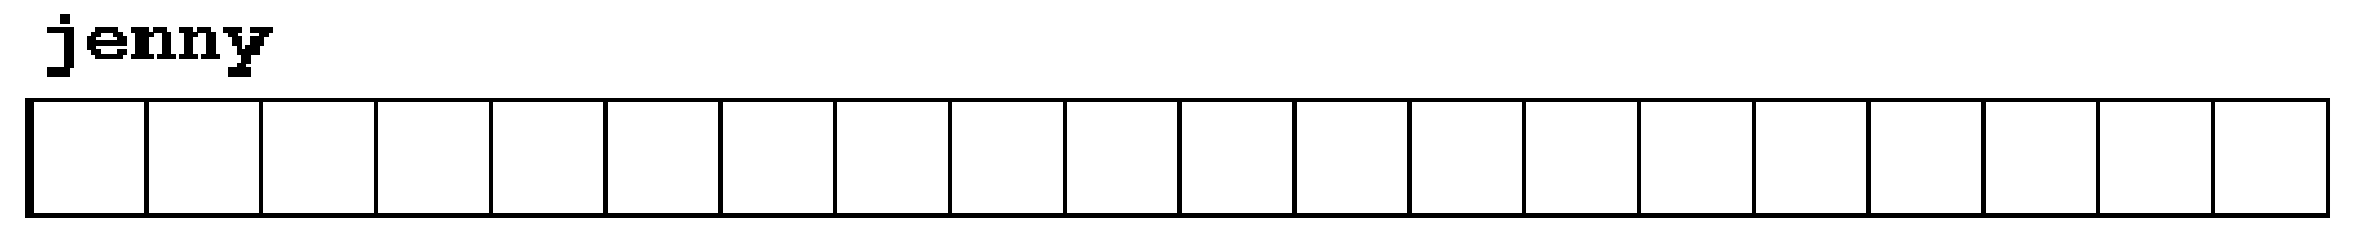
\includegraphics[width=0.5\linewidth]{../pic/3316/29.png}
\end{center}
Our array of 20 elements of type char, called jenny, can be represented storing the characters sequences "Hello" and "Merry Christmas" as:
\begin{center}
	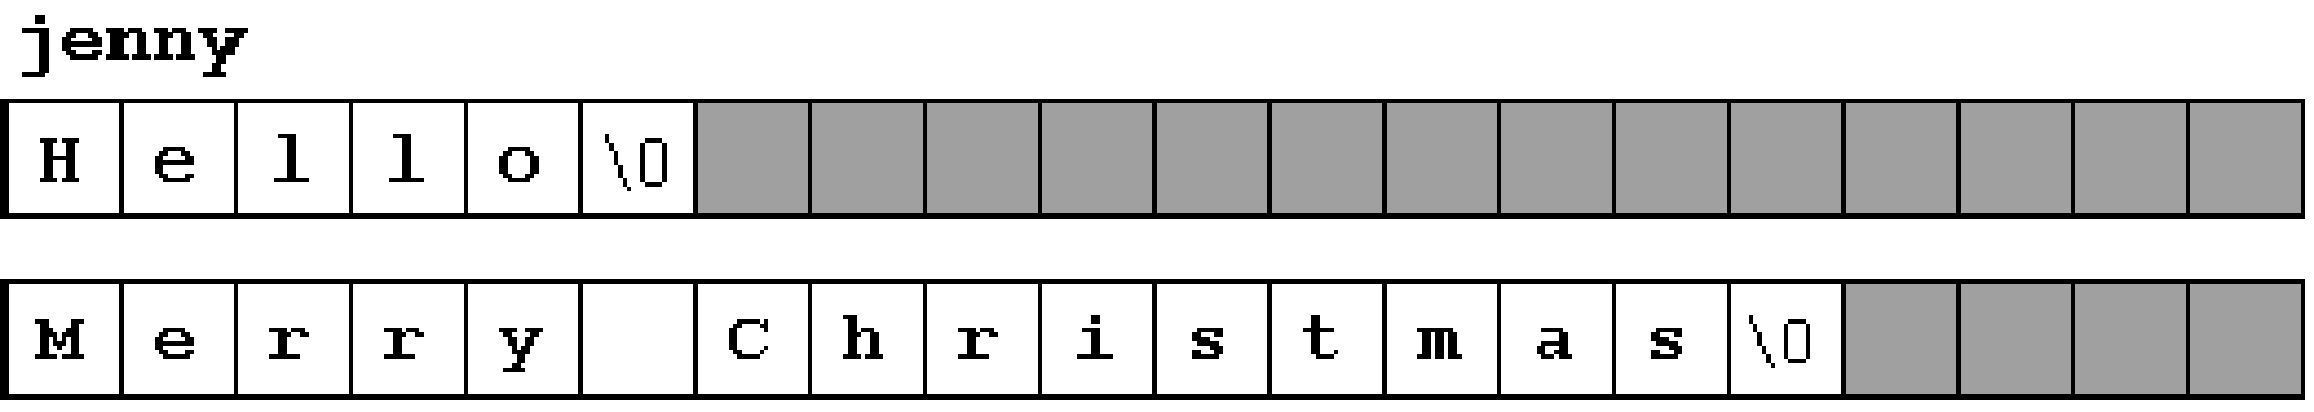
\includegraphics[width=0.5\linewidth]{../pic/3316/30.png}
\end{center}
we can initialize the array of char elements called myword with a null-terminated sequence of characters by either one of these two methods:
\begin{lstlisting}[language=C++]
    char myword [] = { 'H', 'e', 'l', 'l', 'o', '\0' };
    char myword [] = "Hello";
\end{lstlisting}
sequences of characters stored in char arrays can easily be converted into string objects just by using the assignment operator:
\begin{lstlisting}[language=C++]
    string mystring; 
    char myntcs[]="some text";
    mystring = myntcs; 
\end{lstlisting}
\section{Pointers}
The memory of your computer can be imagined as a succession of memory cells, each one of the minimal size that computers manage (one byte). These single-byte memory cells are numbered in a consecutive way, so as, within any block of memory, every cell has the same number as the previous one plus one.\\
\subsection{Reference operator (\&)}
The address that locates a variable within memory is what we call a reference to that variable. This reference to a variable can be obtained by preceding the identifier of a variable with an ampersand sign (\&)
\begin{lstlisting}[language=C++]
    ted = &andy;//This would assign to ted the address of variable andy
\end{lstlisting}
The variable that stores the reference to another variable is what we call a pointer
\subsection{Dereference operator (*)}
Pointers are said to "point to" the variable whose reference they store.\\
Using a pointer we can directly access the value stored in the variable which it points to. To do this, we simply have to precede the pointer's identifier with an asterisk (*)
\begin{lstlisting}[language=C++]
    beth = *ted;// beth equal to value pointed by ted
\end{lstlisting}
\begin{center}
	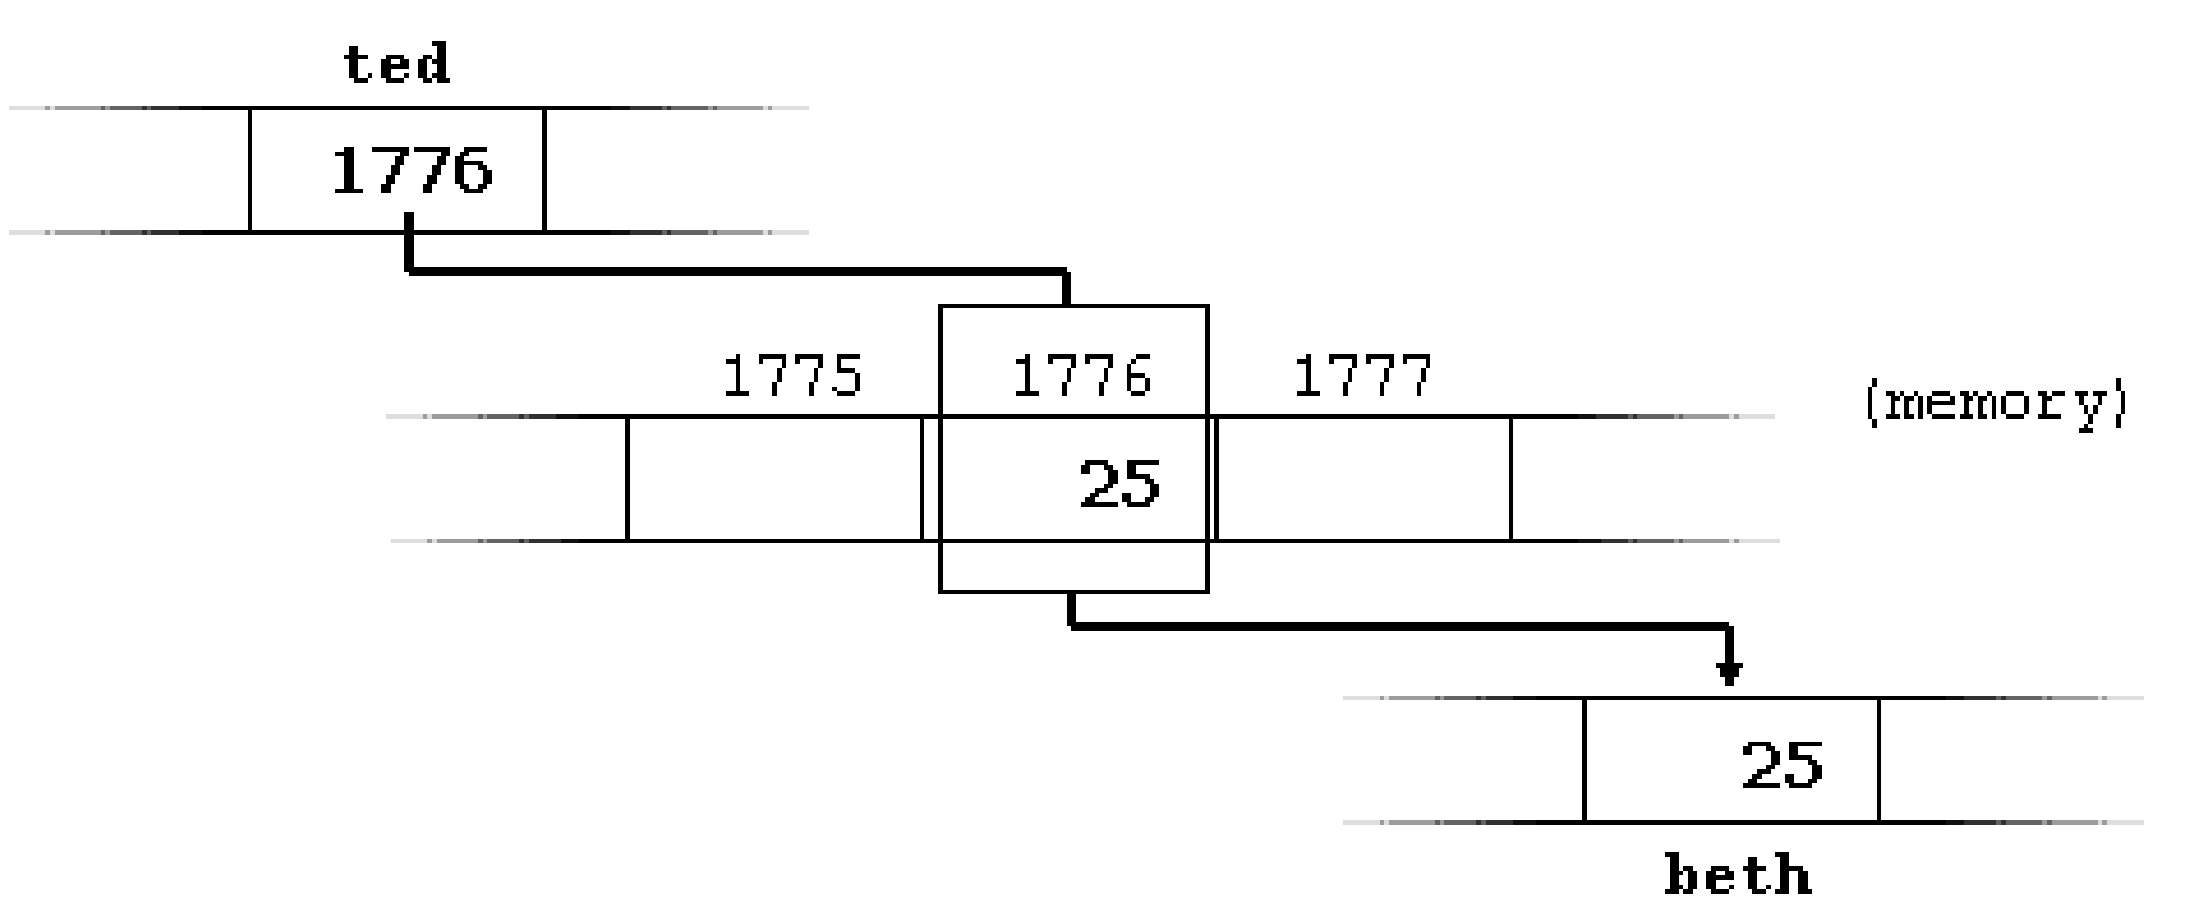
\includegraphics[width=0.5\linewidth]{../pic/3316/31.png}
\end{center}
You must clearly differentiate that the expression ted refers to the value 1776, while *ted refers to the value stored at address 1776
	\begin{lstlisting}[language=C++]
    beth = ted; // beth equal to ted ( 1776 )
    beth = *ted; // beth equal to value pointed by ted ( 25 )
\end{lstlisting}
Notice the difference between the reference and dereference operators:
\begin{itemize}
	\item \& is the reference operator and can be read as "address of"
	\item * is the dereferenece operator and can be read as "value pointed by"
\end{itemize}
Thus, they have complementary (or opposite) meanings. A variable referenced with \& can be dereferenced with *.
	\begin{lstlisting}[language=C++]
    andy = 25; 
    ted = &andy;
    // The following expressions are true
    andy == 25 
    &andy == 1776
    ted == 1776 
    *ted == 25 
    //as long as the address pointed by ted remains unchanged the following expression will be true: 
    *ted == andy
\end{lstlisting}
\subsection{Declaring variables of pointer types}
Due to the ability of a pointer to directly refer to the value that it points to, it becomes necessary to specify in its declaration which data type a pointer is going to point to.\\
The declaraton of pointers :
\begin{lstlisting}[language=C++]
    type * name;
\end{lstlisting}
where type is the data type of the value that the pointer is intended to point to. This type is not the type of the pointer itself! but the type of the data the pointer points to.\\
the asterisk sign (*) that we use when declaring a pointer only means that it is a pointer, and should not be confused with the dereference operator.\\
Declaring multiple pointers
	\begin{lstlisting}[language=C++]
    int * p1, * p2;
\end{lstlisting}
\subsection{Pointers and arrays}
The concept of array is very much bound to the one of pointer. In fact, the identifier of an array is equivalent to the address of its first element, as a pointer is equivalent to the address of the first element that it points to, so in fact they are the same concept.
	\begin{lstlisting}[language=C++]
    int numbers [20];
    int * p; 
    // the following assignment operation would be valid
    p = numbers;
\end{lstlisting}
After that, p and numbers would be equivalent and would have the same properties. The only difference is that we could change the value of pointer p by another one, whereas numbers will always point to the first of the 20 elements of type int with which it was defined. \\
Therefore, unlike p, which is an ordinary pointer, numbers is an array, and an array can be considered a constant pointer.Therefore, the following allocation \underline{would not be valid}:
\begin{lstlisting}[language=C++]
    numbers = p;
\end{lstlisting}
bracket sign operators [] are also a dereference operator known as offset operator. They dereference the variable they follow just as * does, but they also add the number between brackets to the address being dereferenced.
	\begin{lstlisting}[language=C++]
    //These two expressions are equivalent and valid both if a is a pointer or if a is an array.
    a[5] = 0; // a [offset of 5] = 0
    *(a+5) = 0; // pointed by (a+5) = 0
\end{lstlisting}
\subsection{Pointer intialization}
When declaring pointers we may want to explicitly specify which variable we want them to point to:
\begin{lstlisting}[language=C++]
    int number; 
    int *tommy = &number;
    // The behavior of this code is equivalent to 
    int number; 
    int *tommy; 
    tommy = &number;
\end{lstlisting}
When a pointer initialization takes place we are always assigning the reference value to where the pointer points (tommy), never the value being pointed (*tommy).\\
As in the case of arrays, the compiler allows the special case that we want to initialize the content at which the pointer points with constants at the same moment the pointer is declared:
\begin{lstlisting}[language=C++]
    char * terry = "hello";
\end{lstlisting}
In this case, memory space is reserved to contain "hello" and then a pointer to the first character of this memory block is assigned to terry.
\begin{center}
	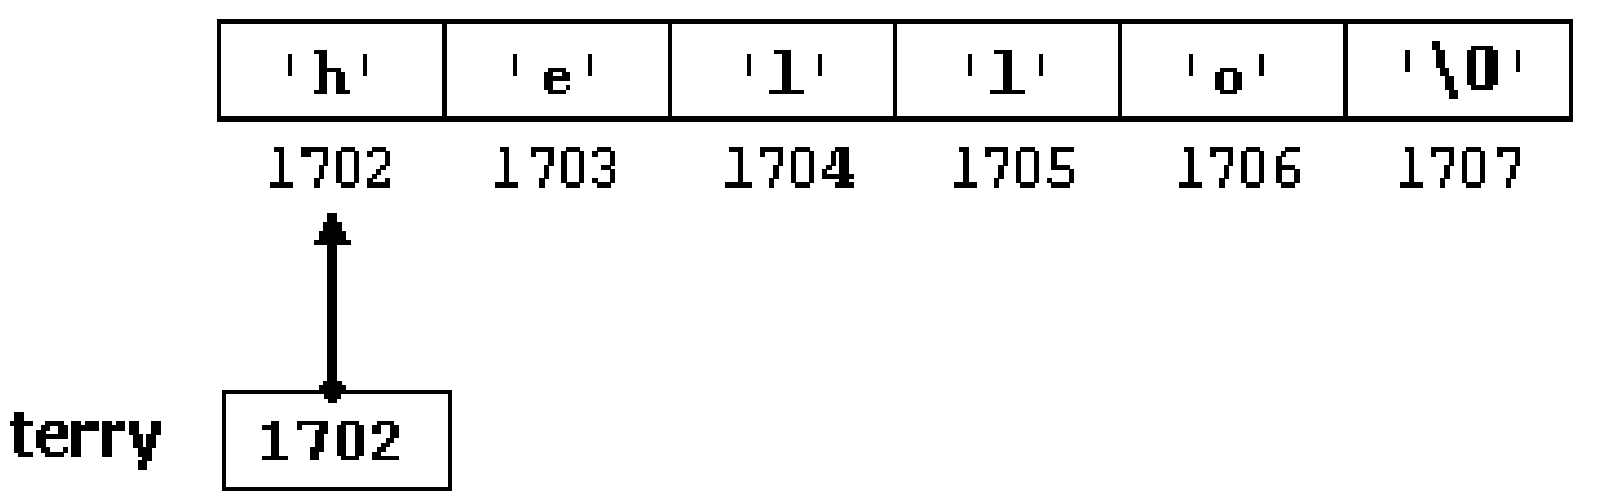
\includegraphics[width=0.5\linewidth]{../pic/3316/32.png}
\end{center}
\begin{center}
	\underline{It is important to indicate that terry contains the value 1702, and not 'h' nor "hello"}
\end{center}
The pointer terry points to a sequence of characters and can be read as if it was an array,we can access the fifth element of the array with any of these two expression:
\begin{lstlisting}[language=C++]
    *(terry+4)
    terry[4] 
\end{lstlisting}
\subsection{Pointer arithmetics}
To conduct arithmetical operations on pointers is a little different than to conduct them on regular integer data types. To begin with, only addition and subtraction operations are allowed to be conducted with them.\\
But both addition and subtraction have a different behavior with pointers according to the size of the data type to which they point.\\

let's assume that in a given compiler for a specific machine, char takes 1 byte, short takes 2 bytes and long takes 4.
	\begin{lstlisting}[language=C++]
    char *mychar;  // point to 1000
    short *myshort;// point to 2000
    long *mylong; // point to 3000

    mychar++; // point to 1001 
    myshort++;// point to 2002 
    mylong++; // point to 3004
    //It would happen exactly the same if we write:
    mychar = mychar + 1; 
    myshort = myshort + 1;
    mylong = mylong + 1; 
\end{lstlisting}
\begin{center}
	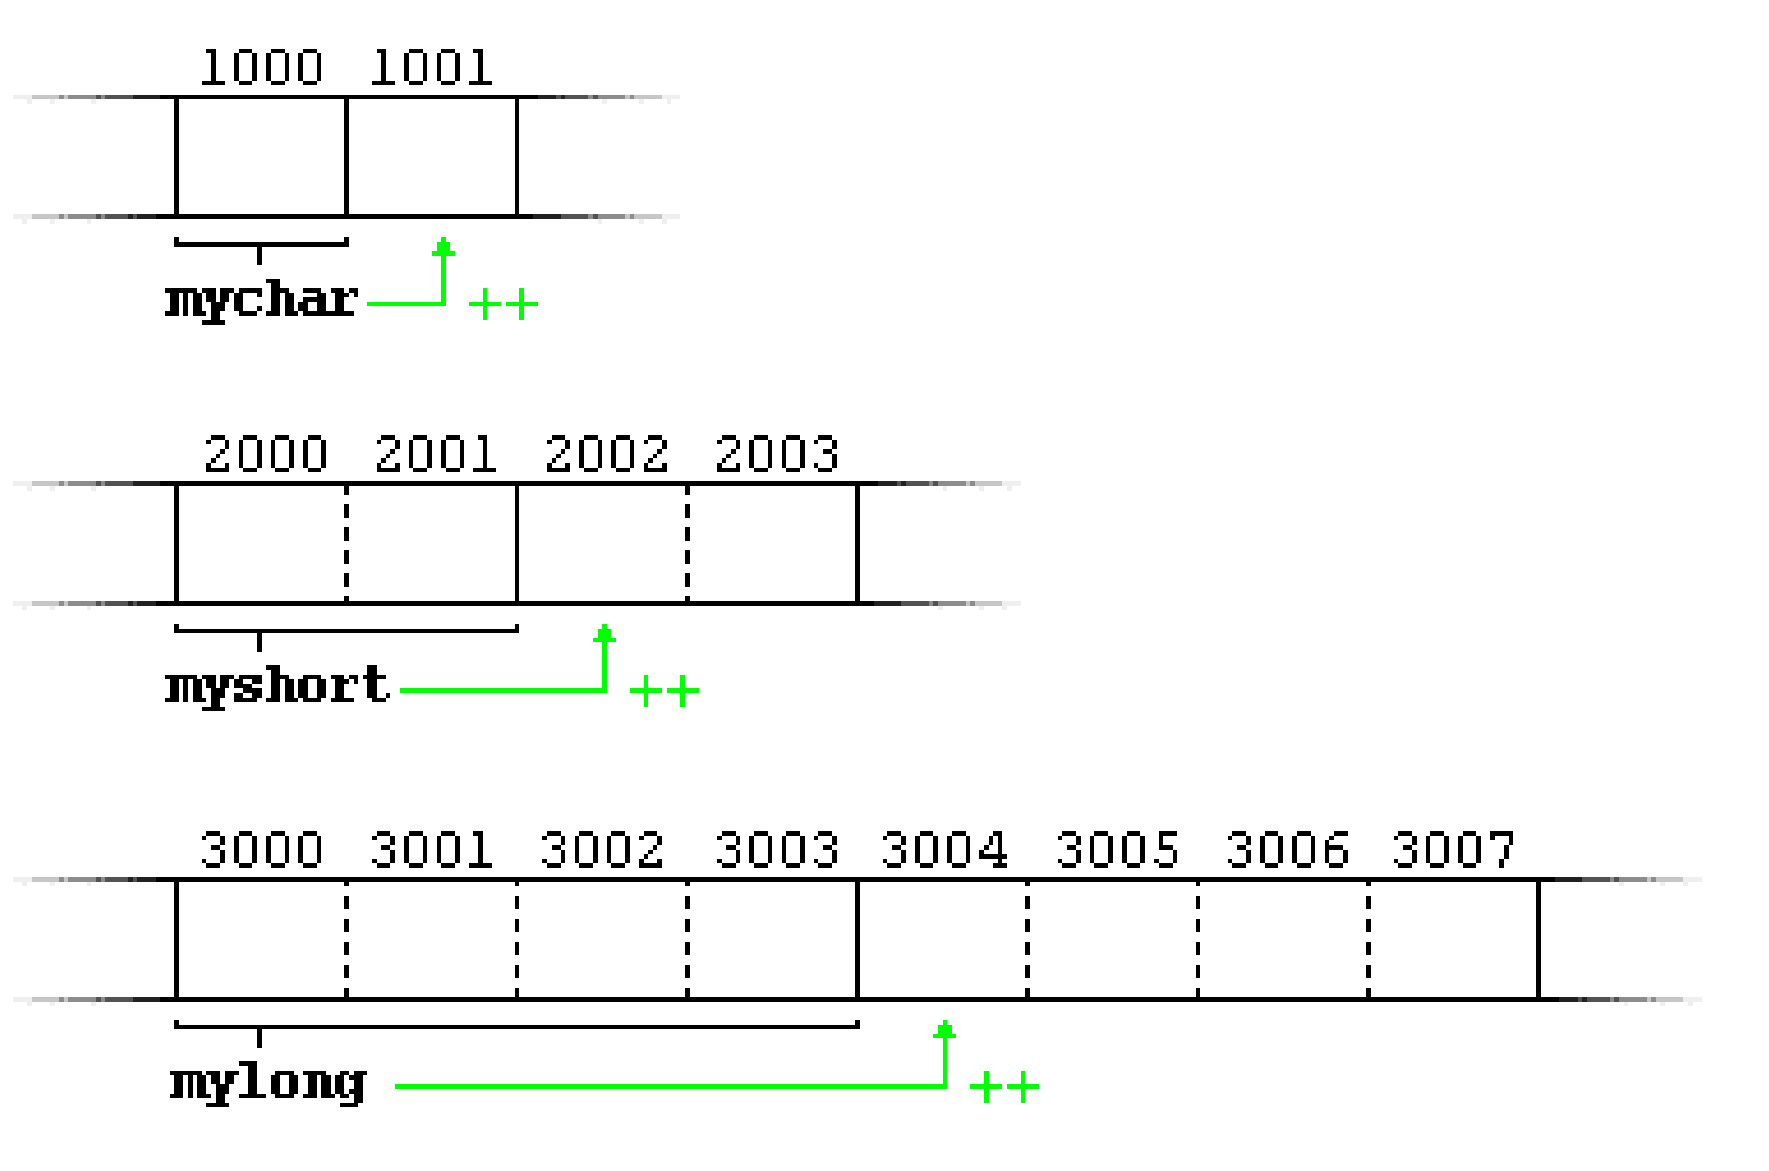
\includegraphics[width=0.5\linewidth]{../pic/3316/33.png}
\end{center}

Both the increase (++) and decrease (--) operators have greater operator precedence than the dereference operator (*). \\
Therefore, the following expression may lead to confusion:
\begin{lstlisting}[language=C++]
    // those expression are equivalent
    *p++ ;
    *(p++);
\end{lstlisting}

If we write :
\begin{lstlisting}[language=C++]
    *p++ = *q++;
    // Because ++ has a higher precedence than * It would be roughly equivalent to: 
    *p = *q;
    ++p; 
    ++q; 
\end{lstlisting}
\subsection{Pointers to pointers }
C++ allows the use of pointers that point to pointers,we only need to add an asterisk (*) for each level of reference in their declarations:
\begin{lstlisting}[language=C++]
    char a; 
    char * b; 
    char ** c;
    a = 'z'; 
    b = &a; 
    c = &b; 
\end{lstlisting}
\begin{center}
	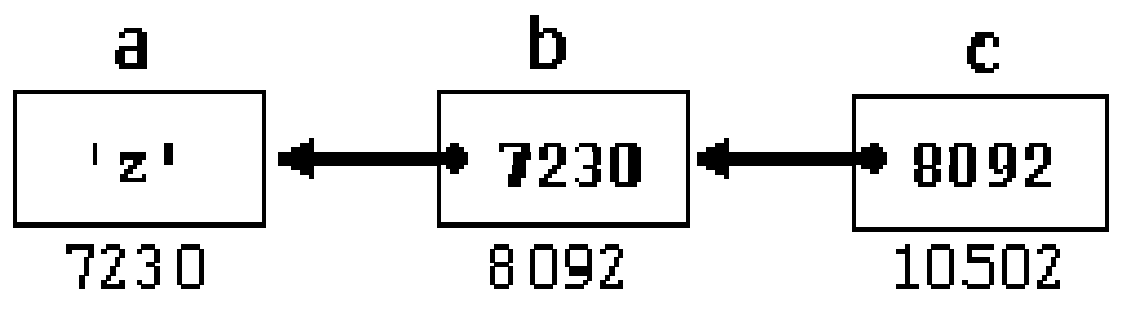
\includegraphics[width=0.5\linewidth]{../pic/3316/34.png}\\
	{\tiny The value of each variable is written inside each cell; under the cells are their respective addresses in memory.}
\end{center}
\begin{itemize}
	\item c has type char** and a value of 8092
	\item *c has type char* and a value of 7230
	\item **c has type char and a value of 'z'
\end{itemize}
\subsection{Void pointers}
The void type of pointer is a special type of pointer. In C++, void represents the absence of type, so void pointers are pointers that point to a value that has no type.\\
This allows void pointers to point to any data type, in exchange he data pointed by them cannot be directly dereferenced.\\
One of its uses may be to pass generic parameters to a function
\subsection{Null pointer}
A null pointer is a value that any pointer may take to represent that it is pointing to "nowhere".
\begin{lstlisting}[language=C++]
    int * p; 
    p = 0; // p has a null pointer value
\end{lstlisting}
\subsection{Pointers to functions }
The ty../pic/3316al use of this is for passing a function as an argument to another function, since these cannot be passed dereferenced.\\
In order to declare a pointer to a function we have to
declare it like the prototype of the function except that the name of the function is enclosed between parentheses () and an asterisk (*) is inserted before the name:
\begin{lstlisting}[language=C++]
#include <iostream>
using namespace std; 
int addition (int a, int b) { return (a+b); } 
int subtraction (int a, int b) { return (a-b); } 
int operation (int x, int y, int(*functocall)(int,int)) { 
int g; 
g = (*functocall)(x,y); 
return (g); 
} 
int main () { 
int m,n; 
int (*minus)(int,int) = subtraction; //minus is a pointer to a function that has two parameters
m = operation (7, 5, addition); 
n = operation (20, m, minus); 
cout <<n; 
return 0; 
} 

Output :
    8
\end{lstlisting}
\section{Dynamic memory}
if we need a variable amount of memory that can only be determined during runtime we must use dynamic memory.
\subsection{Operators new and new[]}
In order to request dynamic memory we use the operator new followed by a data type specifier.\\
It returns a pointer to the beginning of the new block of memory allocated.
	\begin{lstlisting}[language=C++]
pointer = new type //allocate memory to contain one single element
pointer = new type [number_of_elements] //assign a block (an array) of elements of type type,
// exemple 
int * bobby; 
bobby = new int [5];
\end{lstlisting}
The system dynamically assigns space for five elements of type int and returns a pointer to the first element of the sequence, which is assigned to bobby.\\
Therefore, now, bobby points to a valid block of memory with space for five elements of type int.
\begin{center}
	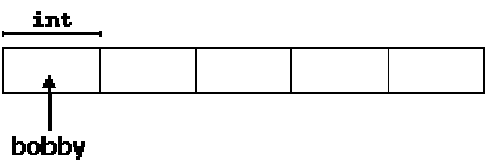
\includegraphics[width=0.5\linewidth]{../pic/3316/36.png}
\end{center}
\subsubsection{Difference between declaring a normal array and assigning dynamic memory to a pointer}
the dynamic memory allocation allows us to assign memory during the execution of the program (runtime) using any variable or constant value as its size.

\subsection{Check if the allocation was successful }
Computer memory is a limited resource, when a memory allocation fails, terminating the program, the pointer returned by new is a null pointer.
	\begin{lstlisting}[language=C++]
int * bobby; 
bobby = new (nothrow) int [5]; 
if (bobby == 0) { 
 // error assigning memory. Take measures.
 }; 
\end{lstlisting}
\subsection{Operators delete and delete[] }
Since the necessity of dynamic memory is usually limited to specific moments within a program, once it is no longer needed it should be freed so that the memory becomes available again.\\
\begin{lstlisting}[language=C++]
delete pointer; //  delete memory allocated for a single element
delete [] pointer;// delete memory allocated for arrays of elements. 
\end{lstlisting}
The value passed as argument to delete must be a pointer to a memory block previously allocated with new.
\section{Data Structure}
A data structure is a group of data elements grouped together under one name. These data elements, known as members, can have different types and different lengths.
	\begin{lstlisting}[language=C++]
struct structure_name { 
    member_type1 member_name1; 
    member_type2 member_name2; 
    member_type3 member_name3; 
    . 
    . 
} object_names; 
\end{lstlisting}
\begin{itemize}
	\item structure\_name is a name for the structure type
	\item Right at the end of the struct declaration, and before the ending semicolon, we can use the optional field object\_name to directly declare objects of the structure type.
\end{itemize}
we have to know is that a data structure creates a new type: Once a data structure is declared, a new type with the identifier specified as structure\_name is created and can be used in the rest of the program
	\begin{lstlisting}[language=C++]
struct product { 
    int weight; 
    float price; 
} ; 
product apple; 
product banana, melon;
\end{lstlisting}

We can use a dot (.) to operate directly with the objects member as if they were standard variables.
	\begin{lstlisting}[language=C++]
    apple.weight 
    apple.price 
    banana.weight
    banana.price 
    melon.weight 
    melon.price 
\end{lstlisting}
\subsection{Pointer to structures}
Like any other type, structures can be pointed by its own type of pointers.\\
The arrow operator ($->$) is a dereference operator that is used exclusively with pointers to objects with members.\\
\begin{lstlisting}[language=C++]
struct movies_t { 
 string title; 
 int year; 
}; 
movies_t amovie; 
movies_t * pmovie;
// the following code would also be valid 
pmovie = &amovie;
// The following code is equivalent to (*pmovie).title
pmovie->year; 
// note that  *pmovie.title is equivalent to *(pmovie.title)
\end{lstlisting}
\subsection{Nesting structures}
Structures can also be nested so that a valid element of a structure can also be in its turn another structure.
	\begin{lstlisting}[language=C++]
struct movies_t { 
    string title; 
    int year; 
}; 
struct friends_t { 
    string name; 
    string email; 
    movies_t favorite_movie; 
 } charlie, maria; 
friends_t * pfriends = &charlie;
// we could use any of the following expressions :
charlie.name 
maria.favorite_movie.title 
// the two following expressions are the same member
charlie.favorite_movie.year 
pfriends->favorite_movie.year
\end{lstlisting}



\chapter{Object Oriented Programming}
\section{Classes}
A class is an expanded concept of a data structure:it can hold both data and functions.\\
An object is an instantiation of a class.
	\begin{lstlisting}[language=C++]
class class_name { 
    access_specifier_1: 
    member1; 
    access_specifier_2: 
    member2; 
    ... 
} object_names;
\end{lstlisting}
The body of the declaration can contain members, that can be either data or function declarations,and optionally access specifiers.\\

An access specifier is one of the following three keywords: private, public or protected. These specifiers modify the access rights that the members following them acquire:
\begin{itemize}
	\item private (accessible from members of the same class), default access.
	\item protected (accessible form members from the same class and from their derived classes)
	\item public (accessible from anywhere)
\end{itemize}
\begin{lstlisting}[language=C++]
class CRectangle { 
    int x, y; 
    public: 
    void set_values (int,int);
    int area (void); 
 } rect; 
\end{lstlisting}
We can to any of the public members of the object as if they were normal functions or normal variables, just by putting the object's name followed by a dot (.) and then the name of the member.\\
\begin{lstlisting}[language=C++]
    rect.set_values (3,4);
    myarea = rect.area(); 
\end{lstlisting}
The two colons "::" is used to define a member of a class from outside the class definition.\\
\begin{lstlisting}[language=C++]
void CRectangle::set_values (int a, int b) { 
 x = a; 
 y = b; 
} 
\end{lstlisting}

\begin{center}\fbox{\begin{minipage}{\linewidth}
			\begin{center}
				That is the basic concept of object-oriented programming: Data and functions are both members of the object.
			\end{center}
		\end{minipage}}\end{center}
\subsection{Constructors and destructors}
\subsubsection{Constructors}
A class can include a special function called constructor, which is automatically called whenever a new object of this class is created.\\
This constructor function must have the same name as the class, and cannot have any return type; not even void.
	\begin{lstlisting}[language=C++]
#include <iostream>
using namespace std; 
class CRectangle { 
 int width, height; 
 public: 
 CRectangle (int,int); 
 int area () {return (width*height);} 
}; 
CRectangle::CRectangle (int a, int b) { 
 width = a; 
 height = b; 
} 
int main () { 
 CRectangle rect (3,4); 
 CRectangle rectb (5,6); 
 cout << "rect area: " << rect.area() << endl; 
 cout << "rectb area: " << rectb.area() << endl; 
 return 0; 
} 
-----------------
Output:
rect area: 12 
rectb area: 30 
\end{lstlisting}
Constructors cannot be called explicitly as if they were regular member functions. They are only executed when a new object of that class is created.
\subsubsection{Overloading}
A constructor can also be overloaded with more than one function that have the same name but different types or number of parameters.
	\begin{lstlisting}[language=C++]
#include <iostream>
using namespace std; 
class CRectangle { 
 int width, height; 
 public: 
 CRectangle (); 
 CRectangle (int,int); 
 int area (void) {return (width*height);} 
}; 
CRectangle::CRectangle () { 
 width = 5; 
 height = 5; 
} 
CRectangle::CRectangle (int a, int b) { 
 width = a; 
 height = b; 
} 
int main () { 
 CRectangle rect (3,4); 
 CRectangle rectb; 
 cout << "rect area: " << rect.area() << endl; 
 cout << "rectb area: " << rectb.area() << endl; 
 return 0; 
}
-------------
Output:
rect area: 12 
rectb area: 25 
\end{lstlisting}
\underline{Important :} Notice how if we declare a new object and we want to use its default constructor (the one without parameters), we do not include parentheses ():
\begin{lstlisting}[language=C++]
    CRectangle rectb; // right
    CRectangle rectb(); // wrong!
\end{lstlisting}
\subsubsection{Default constructor}
The compiler creates a default constructor for you if you do not specify your own. It provides three special member functions in total that are implicitly declared
\begin{itemize}
	\item the copy constructor
	\item the copy assignemnt operator
	\item the default destructor
\end{itemize}
The copy constructor and the copy assignment operator copy all the data contained in another object to the data members of the current object.\\
it would be somthing like
	\begin{lstlisting}[language=C++]
Classname::Classname (const Classname& rv) {
 a=rv.a; b=rv.b; c=rv.c; 
 }
\end{lstlisting}
Therefore
	\begin{lstlisting}[language=C++]
    // using the constructor maded by the programmers
    Classname object1 (2,3); 
    // using the default constructo
    Classname object2 (object1);// we copy the object1
\end{lstlisting}
\subsubsection{Destructor}
The destructor fulfills the opposite functionality. It is automatically called when an object is destroyed, either because its scope of existence has finished or because it is an object dynamically assigned and it is released using the operator delete.\\
The destructor must have the same name as the class, but preceded with a tilde sign ($\sim$) and it must also return no value.\\

The use of destructors is especially suitable when an object assigns dynamic memory during its lifetime and at the moment of being destroyed we want to release the memory that the object was allocated.
	\begin{lstlisting}[language=C++]
#include <iostream>
using namespace std; 
class CRectangle { 
 int *width, *height; 
 public: 
 CRectangle (int,int); 
 ~CRectangle (); 
 int area () {return (*width * *height);} 
}; 
CRectangle::CRectangle (int a, int b) { 
 width = new int; 
 height = new int; 
 *width = a; 
 *height = b; 
} 
CRectangle::~CRectangle () { 
 delete width; 
 delete height; 
} 
\end{lstlisting}
\subsection{Pointers to classes}
A class becomes a valid type, so we can use the class name as the type for the pointer.\\
As it happened with data structures, in order to refer directly to a member of an object pointed by a pointer we can use the arrow operator ($->$) of indirection.
\subsection{Overloading operators}
When you define a class, you are actually creating a new type.\\
Most of the C++ operators can be overloaded to apply to your new class type.
\begin{center}
	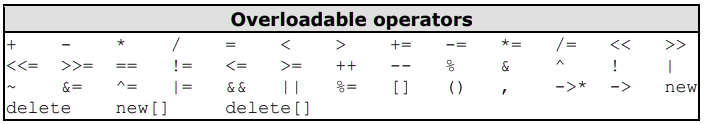
\includegraphics[width=0.5\linewidth]{../pic/3316/35.png}
\end{center}
To overload an operator in order to use it with classes we declare operator functions, which are regular functions whose names are the operator keyword followed by the operator sign that we want to overload.
	\begin{lstlisting}[language=C++]
        type operator sign (parameters) { /*...*/ }
    \end{lstlisting}
Example :
\begin{lstlisting}[language=C++]
// vectors: overloading operators example
#include <iostream>
using namespace std; 
class CVector { 
 public: 
 int x,y; 
 CVector () {}; 
 CVector (int,int); 
 CVector operator + (CVector); 
}; 
CVector::CVector (int a, int b) { 
 x = a; 
 y = b; 
} 
CVector CVector::operator+ (CVector param) { 
 CVector temp; 
 temp.x = x + param.x; 
 temp.y = y + param.y; 
 return (temp); 
} 
int main () { 
 CVector a (3,1); 
 CVector b (1,2); 
 CVector c; 
 c = a + b; 
 cout << c.x << "," << c.y; 
 return 0; 
}
--------------
Output : 
4,3
\end{lstlisting}
Both expressions are equivalent :
\begin{lstlisting}[language=C++]
    c = a + b; 
    c = a.operator+ (b);
\end{lstlisting}
\subsection{The keyword this}
The keyword this represents a pointer to the object whose member function is being executed. It is a pointer to the object itself. \\
Example :
\begin{lstlisting}[language=C++]
#include <iostream>
using namespace std; 
class CDummy { 
 public: 
 int isitme (CDummy& param); 
}; 
int CDummy::isitme (CDummy& param) 
{ 
 if (&param == this) return true; 
 else return false; 
} 
int main () { 
 CDummy a; 
 CDummy* b = &a; 
 if ( b->isitme(a) ) 
 cout << "yes, &a is b"; 
 return 0; 
} 
\end{lstlisting}
\subsection{Static members }
Static data members of a class are also known as "class variables", because there is only one unique value for all the objects of that same class. Their content is not different from one object of this class to another. \\
it may be used for a variable within a class that can contain a counter with the number of objects of that class that are currently allocated
	\begin{lstlisting}[language=C++]
#include <iostream>
using namespace std; 
class CDummy { 
 public: 
 static int n; 
 CDummy () { n++; }; 
 ~CDummy () { n--; }; 
}; 
int CDummy::n=0; 
int main () { 
 CDummy a; 
 CDummy b[5]; 
 CDummy * c = new CDummy; 
 cout << a.n << endl; 
 delete c; 
 cout << CDummy::n << endl; 
 return 0; 
} 
\end{lstlisting}
In fact, static members have the same properties as global variables but they enjoy class scope.\\
we can only include the prototype (its declaration) in the class declaration but not its definition (its initialization).\\
In order to initialize a static data-member we must include a formal definition outside the class.
\chapter{Input/Output with files}
C++ provides the following classes to perform output and input of characters to/from files:
\begin{itemize}
	\item ofstream: Stream class to write on files.
	\item ifstream: Stream class to read from files.
	\item fstream: Stream class to both read and write from/to files.
\end{itemize}
\section{Open a file}
In order to open a file with a stream object we use its member function open():
\begin{lstlisting}[language=C++]
    open (filename,mode);
\end{lstlisting}
Where filename representing the name of the file to be opened and mode is an optional parameter with a combination of the following flags: \\
\begin{tabular}{|l|l|}
	\hline
	\specialcell{ios::in}     & \specialcell{Open for input operations. }                                                           \\ \hline
	\specialcell{ios::out}    & \specialcell{Open for output operations.}                                                           \\ \hline
	\specialcell{ios::binary} & \specialcell{Open in binary mode.}                                                                  \\ \hline
	\specialcell{ios::ate}    & \specialcell{Set the initial position at the end of the file. If this flag is not set to any value, \\ the initial position is the beginning of the file.}   \\ \hline
	\specialcell{ios::app}    & \specialcell{All output operations are performed at the end of the file,                            \\ appending the content to the current content  of the file.\\ This flag can only be used in streams open for output-only operations.}   \\ \hline
	\specialcell{ios::trunc}  & \specialcell{If the file opened for output operations already existed before,                       \\its previous content is deleted and replaced by the new one.}   \\ \hline
\end{tabular}\\
All these flags can be combined using the bitwise operator OR (|).
Each one of the open() member functions of the classes ofstream, ifstream and fstream has a default mode that is used if the file is opened without a second argument: \\
\begin{tabular}{|l|l|}
	\hline
	ofstream & ios::out             \\ \hline
	ifstream & ios::in              \\ \hline
	fstream  & ios::in $|$ ios::out \\ \hline
\end{tabular}\\
Note that : File streams opened in binary mode perform input and output operations independently of any format considerations.\\

To check if a file stream was successful opening a file, you can do it by calling to member is\_open()
\begin{lstlisting}[language=C++]
    if (myfile.is_open()) { /* ok, proceed with output */ }
\end{lstlisting}
\section{Closing a file}
When we are finished with our input and output operations on a file we shall close it so that its resources become available again.\\
In order to do that we have to call the stream's member function close().
	\begin{lstlisting}[language=C++]
    myfile.close();
\end{lstlisting}
In case that an object is destructed while still associated with an open file, the destructor automatically calls the member function close().
\section{Text files}
Text file streams are those where we do not include the ios::binary flag in their opening mode.
\subsection{Writing on a text file}
\begin{lstlisting}[language=C++]
#include <iostream>
#include <fstream>
using namespace std; 
int main () { 
 ofstream myfile ("example.txt"); 
 if (myfile.is_open()) 
 { 
 myfile << "This is a line.\n"; 
 myfile << "This is another line.\n"; 
 myfile.close(); 
 } 
 else cout << "Unable to open file"; 
 return 0; 
} 
\end{lstlisting}
\subsection{ reading a text file}
\begin{lstlisting}[language=C++]
#include <iostream>
#include <fstream>
#include <string>
using namespace std; 
int main () { 
 string line; 
 ifstream myfile ("example.txt"); 
 if (myfile.is_open()) 
 { 
 while (! myfile.eof() ) 
 { 
 getline (myfile,line); 
 cout << line << endl; 
 } 
 myfile.close(); 
 } 
 else cout << "Unable to open file"; 
 return 0; 
}
\end{lstlisting}
The function eof() returns true in the case that the end of the file has been reached.
\end{document}